\documentclass[../../main]{subfiles}

\renewcommand\thesection{\arabic{section}}


\begin{document}

\section{Multiplexer System} \label{sec:}

Now let's focus on the \emph{sensing} part, we will have outputs from different
\emph{sensor modules} and \emph{feedback} from all the \emph{actuators}\footnote{right now
actuator feedback is not implemented.}. So we need a way to gather all these information
for the \esp to process.

The design requirements are:

\begin{itemize}
    \item It should be analog, because we will need to read voltage values.
    \item It should be bi-directional, because the communication to DHT22 sensor\footnote{the
        sensor used for sensing temperature and humidity.} is done via a single pin.
    \item It should have two separately controllable multiplexer units. It would give us
        more flexibility and can be used to communicate with devices that require two
        pins. For example, the ultrasonic sensor \emph{HC-SR04}\footnote{right now we are
        not using the sensor but we need it to measure the reservoir level in the future},
        which requires two pins for communication.
    \item The pins required to operate should be minimum as possible.
\end{itemize}

So first of all, we need an \emph{analog multiplexer}. The difference between a \emph{digital
multiplexer} and an \emph{analog multiplexer} is that, the former one generates the output
from the inputs using logic gates, and the latter directly connects\footnote{usually using
\emph{transmission gates}.} the inputs to the output depending on the select lines.

The output of the \emph{digital multiplexer} will be always either be high or low. But in
the case of \emph{analog multiplexer} the output is directly tied to the selected input
through a \emph{transmission gate}. Hence the latter is also \emph{bi-directional} in nature,
and can act as a \emph{demultiplexer}.

\alertNote{
    Also note that the \emph{analog multiplexer} can be used as a \emph{digital multiplexer}.
}

For future proofing, let the input count of a single multiplexer set be $32$. That means the
each set of multiplexer will take a $5$ bit address, and can \emph{read} / \emph{write} to
$32$ different \emph{source} / \emph{destination}. That would give us the ability to connect
almost $64$\footnote{given that every sensor uses a single pin to communicate.} different
\emph{sensors} to the \esp. And can simultaneously use $2$ different \emph{source} / \emph{destination}.

An ideal candidate for our design is \emph{74HC4067}, which is a $16$ bit
\emph{analog multiplexer / demultiplexer} with an \emph{active low} enable. Please refer figures
\ref{fig:74hc4067Smd} and \ref{fig:74hc4067PinDiagram} for more information. And refer table
\ref{tbl:74hc4067RelventPins} for the information about relevant pins.

\begin{center}
    {\begin{minipage}[c] {0.42\textwidth}
        \centering
        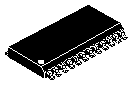
\includegraphics [
        ] {pics/74hc4067_smd.pdf}
        \captionof{figure} {
            Smd package of \emph{74HC4067}.
            \label{fig:74hc4067Smd}
        }

        \includegraphics [
            max width = \IGXMaxWidth,
            max height = \IGXMaxHeight,
            \IGXDefaultOptionalArgs,
        ] {tikzpics/endAbsSixteenBitMuxPinout.pdf}
        \captionof{figure} {
            \label{fig:}
        }

    \end{minipage}
    \begin{minipage}[c] {0.52\textwidth}



        %\begin{tabularx} {\linewidth} {
        %        *{1}{>{\centering\arraybackslash}m{0.5\linewidth}}
        %        *{1}{>{\centering\arraybackslash}m{0.5\linewidth}}
        %    }
        %    \toprule
        %    Parameter & Value \\
        %    \midrule
        %    $\si{V}_{CEO}$ Max. & $45 \si{V}$ \\
        %    $\si{V}_{EBO}$ Max. & $6 \si{V}$ \\
        %    $\si{I}_{C}$ Max. & $100 \si{mA}$ \\
        %    $\si{P}_{C}$ Max. & $500 \si{mW}$ \\
        %    $\si{C}_{ob}$ (Output Capacitance) Max. & $6 \si{pF}$ \\
        %    \bottomrule
        %\end{tabularx}
        %\captionof{table} {
        %    Brief specification of \textbf{BC547}.
        %    \label{tbl:bc547Spec}
        %}

    \end{minipage}}

\end{center}

\end{document}
